\documentclass{aes2e}

% Metadata Information
\jyear{2016}
\jmonth{January}
\jvol{1}
\jnum{1}

\usepackage{color}
\newcommand{\gregoire}[1]{\textcolor{red}{Gregoire : #1}}
\newcommand{\mathias}[1]{\textcolor{green}{Mathias : #1}}
\newcommand{\ml}[2][]{\textcolor{blue}{#1 #2}}

%\renewcommand{\baselinestretch}{1.5}

\begin{document}
%
% --- Author Metadata here ---
%\CopyrightYear{2007} % Allows default copyright year (20XX) to be over-ridden - IF NEED BE.
%\crdata{0-12345-67-8/90/01}  % Allows default copyright data (0-89791-88-6/97/05) to be over-ridden - IF NEED BE.
% --- End of Author Metadata ---

\title{Semantic browsing of sound databases \\ without keywords}
%\subtitle{[Extended Abstract]
%\titlenote{A full version of this paper is available as
%\textit{Author's Guide to Preparing ACM SIG Proceedings Using
%\LaTeX$2_\epsilon$\ and BibTeX} at
%\texttt{www.acm.org/eaddress.htm}}}
%
% You need the command \numberofauthors to handle the 'placement
% and alignment' of the authors beneath the title.
%
% For aesthetic reasons, we recommend 'three authors at a time'
% i.e. three 'name/affiliation blocks' be placed beneath the title.
%
% NOTE: You are NOT restricted in how many 'rows' of
% "name/affiliations" may appear. We just ask that you restrict
% the number of 'columns' to three.
%
% Because of the available 'opening page real-estate'
% we ask you to refrain from putting more than six authors
% (two rows with three columns) beneath the article title.
% More than six makes the first-page appear very cluttered indeed.
%
% Use the \alignauthor commands to handle the names
% and affiliations for an 'aesthetic maximum' of six authors.
% Add names, affiliations, addresses for
% the seventh etc. author(s) as the argument for the
% \additionalauthors command.
% These 'additional authors' will be output/set for you
% without further effort on your part as the last section in
% the body of your article BEFORE References or any Appendices.

% of EIGHT authors. SIX appear on the 'first-page' (for formatting
% reasons) and the remaining two appear in the \additionalauthors section.
%

%Author Info.
\authorgroup{
\author{Gr\'egoire Lafay$^1$}, \author{Nicolas Misdarris$^2$},
\author{Mathieu Lagrange$^1$}, \author{Mathias Rossignol$^2$}
\email{(gregoire.lafay@irccyn.ec-nantes.fr)}
\affil{IRCCyN, Ecole Centrale de Nantes $^1$ \quad\quad\quad\quad IRCAM, STMS, UPMC $^2$}
}


%\author{
%\alignauthor
% Gregoire Lafay\\
%       \affaddr{IRCCyN, Ecole Centrale de Nantes}\\
%       \affaddr{1 rue de la Noe}\\
%       \affaddr{Nantes, France} 
%       %\email{gregoire.lafay@irccyn.ec-nantes.fr} 
%\alignauthor 
% Nicolas Misdarris\\
%       \affaddr{IRCAM}\\
%       \affaddr{1 Place Igor\-Stravinsky}\\
%       \affaddr{Paris, France} \\
%       \email{}
%\and
%\alignauthor 
%Mathieu Lagrange\\
%       \affaddr{IRCCyN, Ecole Centrale de Nantes}\\
%       \affaddr{1 rue de la Noe}\\
%       \affaddr{Nantes, France} \\
%\alignauthor 
% Mathias Rossignol\\
%       \affaddr{IRCAM}\\
%       \affaddr{1 Place Igor\-Stravinsky}\\
%       \affaddr{Paris, France} \\
%       \email{}
%}       


% There's nothing stopping you putting the seventh, eighth, etc.
% author on the opening page (as the 'third row') but we ask,
% for aesthetic reasons that you place these 'additional authors'
% in the \additional authors block, viz.
%\additionalauthors{Additional authors: John Smith (The Th{\o}rv{\"a}ld Group,
%email: {\texttt{jsmith@affiliation.org}}) and Julius P.~Kumquat
%(The Kumquat Consortium, email: {\texttt{jpkumquat@consortium.net}}).}
\date{26 December 2014 }
% Just remember to make sure that the TOTAL number of authors
% is the number that will appear on the first page PLUS the
% number that will appear in the \additionalauthors section.

\maketitle

\begin{abstract}
In this paper, we study the relevance of a semantic organization of sounds for easing the browsing of a sound database. For such task, the semantic organization is traditionally hold thanks to a keyword selection process. However, various issues of written language like word polysemy, ambiguities translation issues may bias the browsing process.

We consider here two display of sounds that are organized by considering underlying semantic information that draws a hierarchy. For the sake of comparison, we also consider a display whose organization of sound in the plane is based on acoustic cues. Those three displays are evaluated in terms of search speed in a crowd sourcing experiment. Results 
\end{abstract}

%% A category with the (minimum) three required fields
%\category{H.2.8}{Database Management}{Database Applications}[Data mining]
%%%A category including the fourth, optional field follows...
%\category{D.2.8}{Software Engineering}{Metrics}[complexity measures, performance measures]

%\terms{Design, Experimentation, Human Factors}

\keywords{Audio content management and display, Semantic sound data mining}

\section{Introduction}

With the growing capability of recording and storage, the problem of indexing large databases of audio has recently been the object of much attention \cite{Wold1996}. Most of that effort is dedicated to the automatic inference of indexing metadata from the actual audio recording \cite{Zhang1999, tzanetakis2002musical}; in contrast, the ability to browse such databases in an effective manner has been less considered.


Most media assets management are based on keyword-driven queries. The user enters a word which characterizes the desired item, and the interface presents him with items related to this word. The effectiveness of this principle is primarily based on the typological structure and nomenclature of the database. However, for databases and more specifically for databases of sounds, issues arise:

\begin{enumerate}
\item Sounds, as many others things, can be described in many ways. Sound may be designated by their
sources (a car door), as well as by the action of those sources (the slamming of a car door) or their environments (slamming a car door in a garage) \cite{houix2012lexical, niessen2010categories, brown2011towards}. Designing an effective keyword-based search system requires an accurate description of each sound, which has to be adaptable to the sound representation of each user.
\item Pre-defined verbal descriptions of the sounds made available to the users may potentially bias their browsing and final selection.
\item Localization of the query interface is made difficult as the translation of some words referring to qualitative aspects of the sound such as its ambiance is notoriously ambiguous and subject to cultural specificities.
\item Unless considerable time and resources are invested into developing a multilingual interface, any system based on verbal descriptions can only be used with reduced performance by non-native speakers of the chosen language.
\end{enumerate}

To circumvent those issues, not relying on keywords is desirable. That said, semantics, which is traditionally conveyed through written text, may be important for easing browsing.  

To study this issue, we consider in this paper several means of displaying sounds without relying on any textual representation. One, considered as a reference baseline, do not rely on any semantic information as the sounds are organized according to their acoustical properties, \textit{i.e.} time averaged spectral features. The second one 

Their effectiveness is studied with a search-based task whose aim is find a target sound by browsing the database using the display under evaluation.

The paper is organized as follows: in Section \ref{previous} previous work on the topic of sound database browsing is reviewed. Then, the corpus used in this study is described in Section \ref{dataset}. the three displays under evaluation are next described in Section \ref{display}. The crowd sourcing test used to compare those displays is presented in Section \ref{test}. the outcomes of this experiment are discussed in Section \ref{results}.  

\section{Previous work} \label{previous}

Most of the research effort in Sound Design and Music Information Retrieval (MIR) communities is focused on acoustical based indexing and browsing \cite{tzanetakis2003musescape, streich2008music}. Typically, the items (sound effects or pieces of music) are modeled by processing the digital audio waveform using some signal processing pipeline in order to get a compact description for each  items
\cite{coleman2007mused}. Then, statistical projections or embedding techniques, like Principal components analysis (PCA),  Multi Dimensional Scaling (MDS) \cite{schwarz2009sound,Cano2002}, Self Organizing Maps (SOM) \cite{pampalk2004exploring} and the like are used to project the items in a two or three dimensional space while preserving as much as possible distances among items. One of the advantage of such an approach is its ability to scale to very large databases \cite{schwarz2009scalability} as it does not need any kind of manual annotations and allows to search by similarity efficiently according to acoustical properties.

Though, such acoustical models are inherently subject to observation noise and biases. Selecting the most relevant features to achieve the correct projection of the data may only be performed by an expert user. If done \textit{a priori} by an expert or by some above cited dimensionality reduction technique, the induced bias can strongly limit the user in its ability to . In that respect, semantic tags, if available for the data at hand have the advantage of implicitly structuring the similarity space, thus eventually easing the browsing process even if the actual tags are not -- as in this study -- exposed to the user.

\section{Dataset} \label{dataset}

The interface framework requires a pre-organization of the sound dataset it has to display. This organization is based on semantic considerations. A sound is characterized by a tag describing the source of the sound (\textit{man-yelling}, \textit{car-passing}). Sounds are then grouped into classes according to their tags (\textit{car} $>$ \textit{car-passing}; car $>$ \textit{car-starting}). Those classes are in turn  packed into classes until high level classes describing broad concepts are reached (\textit{traffic} $>$ \textit{car} $>$ \textit{car-passing}). The sound dataset is organized into a hierarchical structure of semantic classes as described in Figure~\ref{figdataset}. The different levels of this hierarchy are called semantic levels. Strictly speaking, the sound samples of the dataset are the leaf semantic levels. All the other classes are represented by a \textit{prototype sound} that best characterizes the sounds belonging to the class. 

That description implies that there are as many leaf classes as sounds in the dataset, which would be unrealistic for large datasets. We therefore propose, in that case, to adapt the organization by considering the leaf classes as \textit{collections} of semantically similar sound samples. Thus, two sounds of \textit{male-yelling} would be grouped into a  single leaf class with the tag \textit{male-yelling}. The leaf class would then also have a \textit{prototype sound} being the most representative item of the different \textit{male-yelling} sounds belonging to the leaf class.

In order for the semantic hierarchical structure to be perceptually valid, the \textit{tags} describing the classes  were chosen from the names of sound categories found by studies addressing environmental auditory scenes perception \cite{niessen2010categories, brown2011towards, dubois2006cognitive}. In cognitive psychology, sound categories may be regarded as intermediaries between collective sound representations and individual sensory experiences \cite{dubois2006cognitive}. It is our belief that using such category names to build the hierarchical structure makes the latter perceptually motivated, and thus meaningful for the users.


%We choose to represent each sound leaf class of our sound data set with a circle. Circles are dispatched in a 2D space and packed together according to the hierarchical structure of the sound set (see figure \ref{SSF}). The class is identified by listening to an acoustic prototype chosen by the authors for its representativeness. Clicking on a circle fires this audio prototype.

\section{Displays} \label{display}

\begin{figure}[t]
\begin{center}
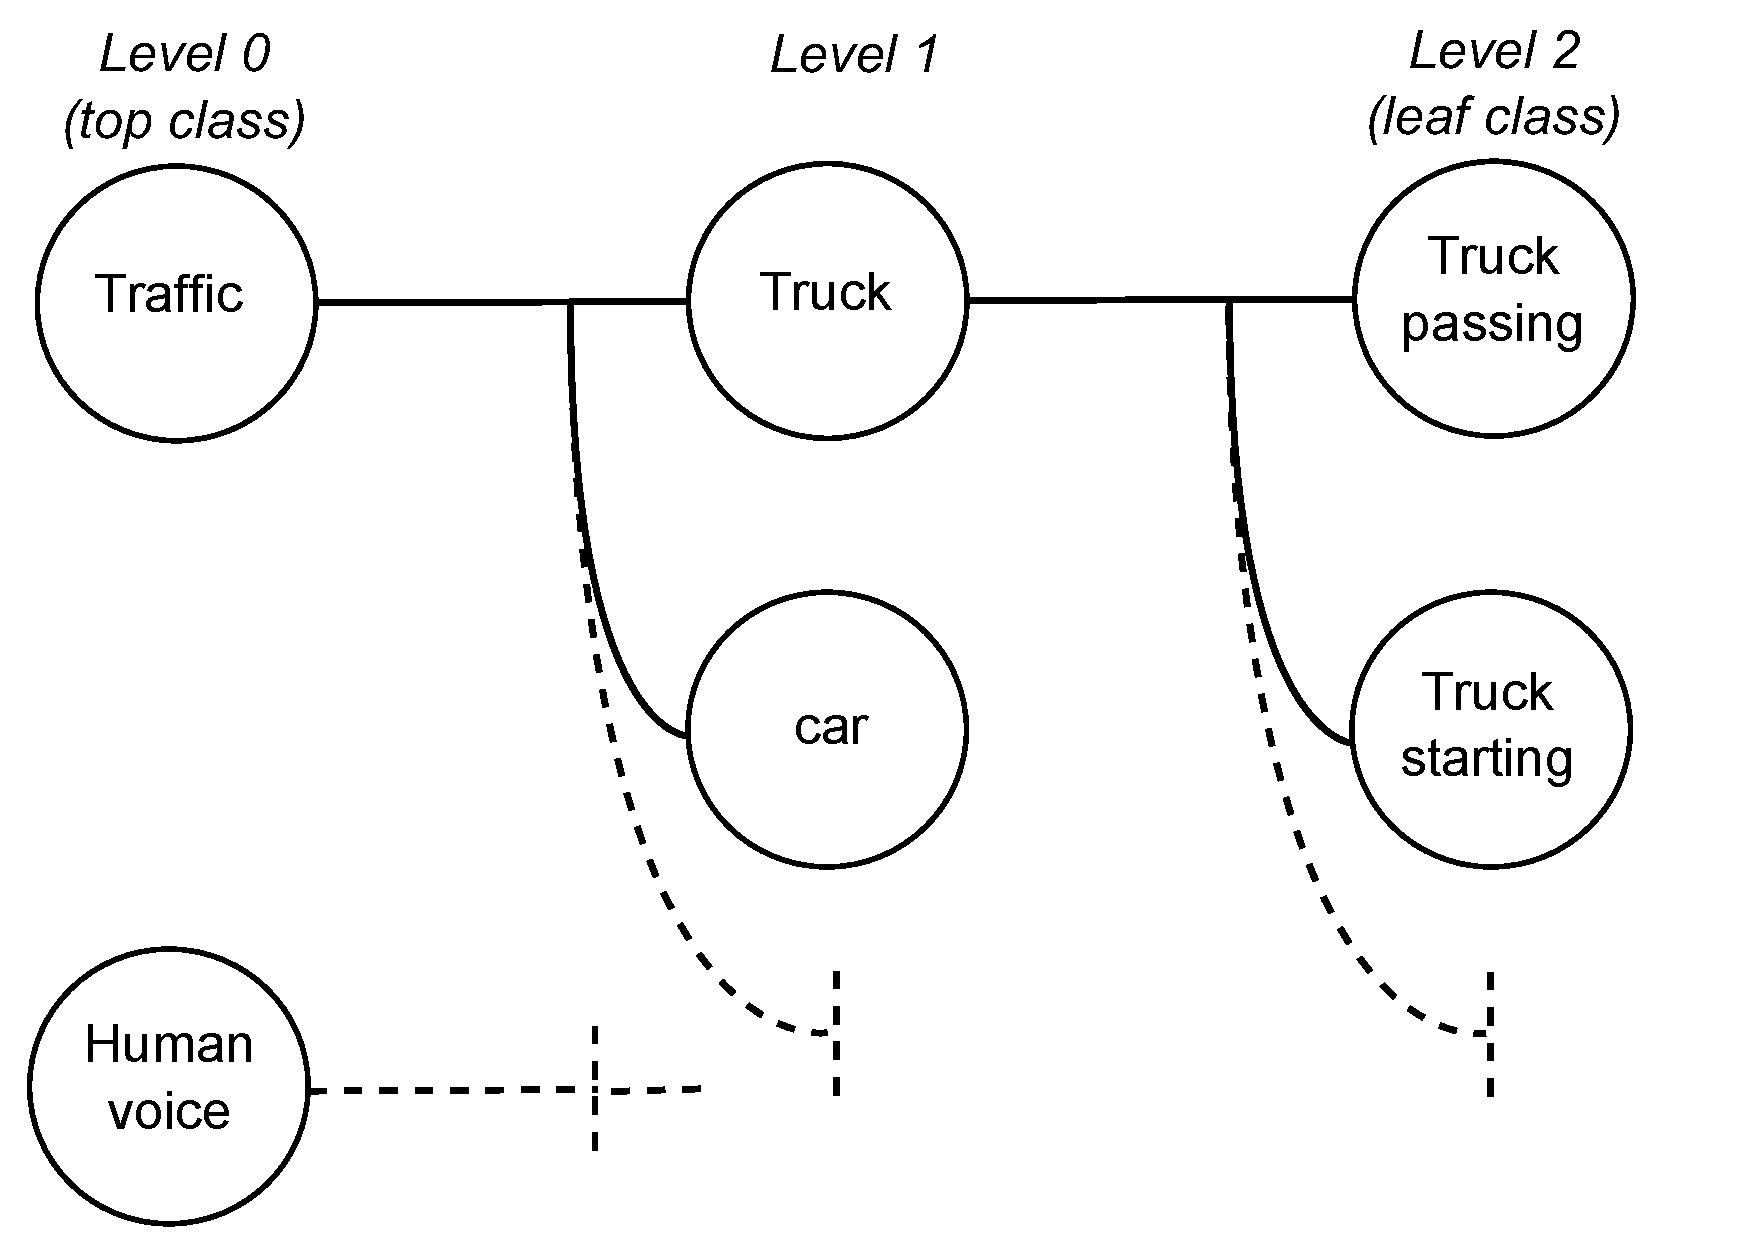
\includegraphics[scale=0.24]{gfx/dataset.pdf} 
\end{center}
\caption{\label{figdataset} Semantic hierarchical structure of the dataset of urban environmental sounds}
\end{figure}




\begin{figure}[t!]
\begin{center}
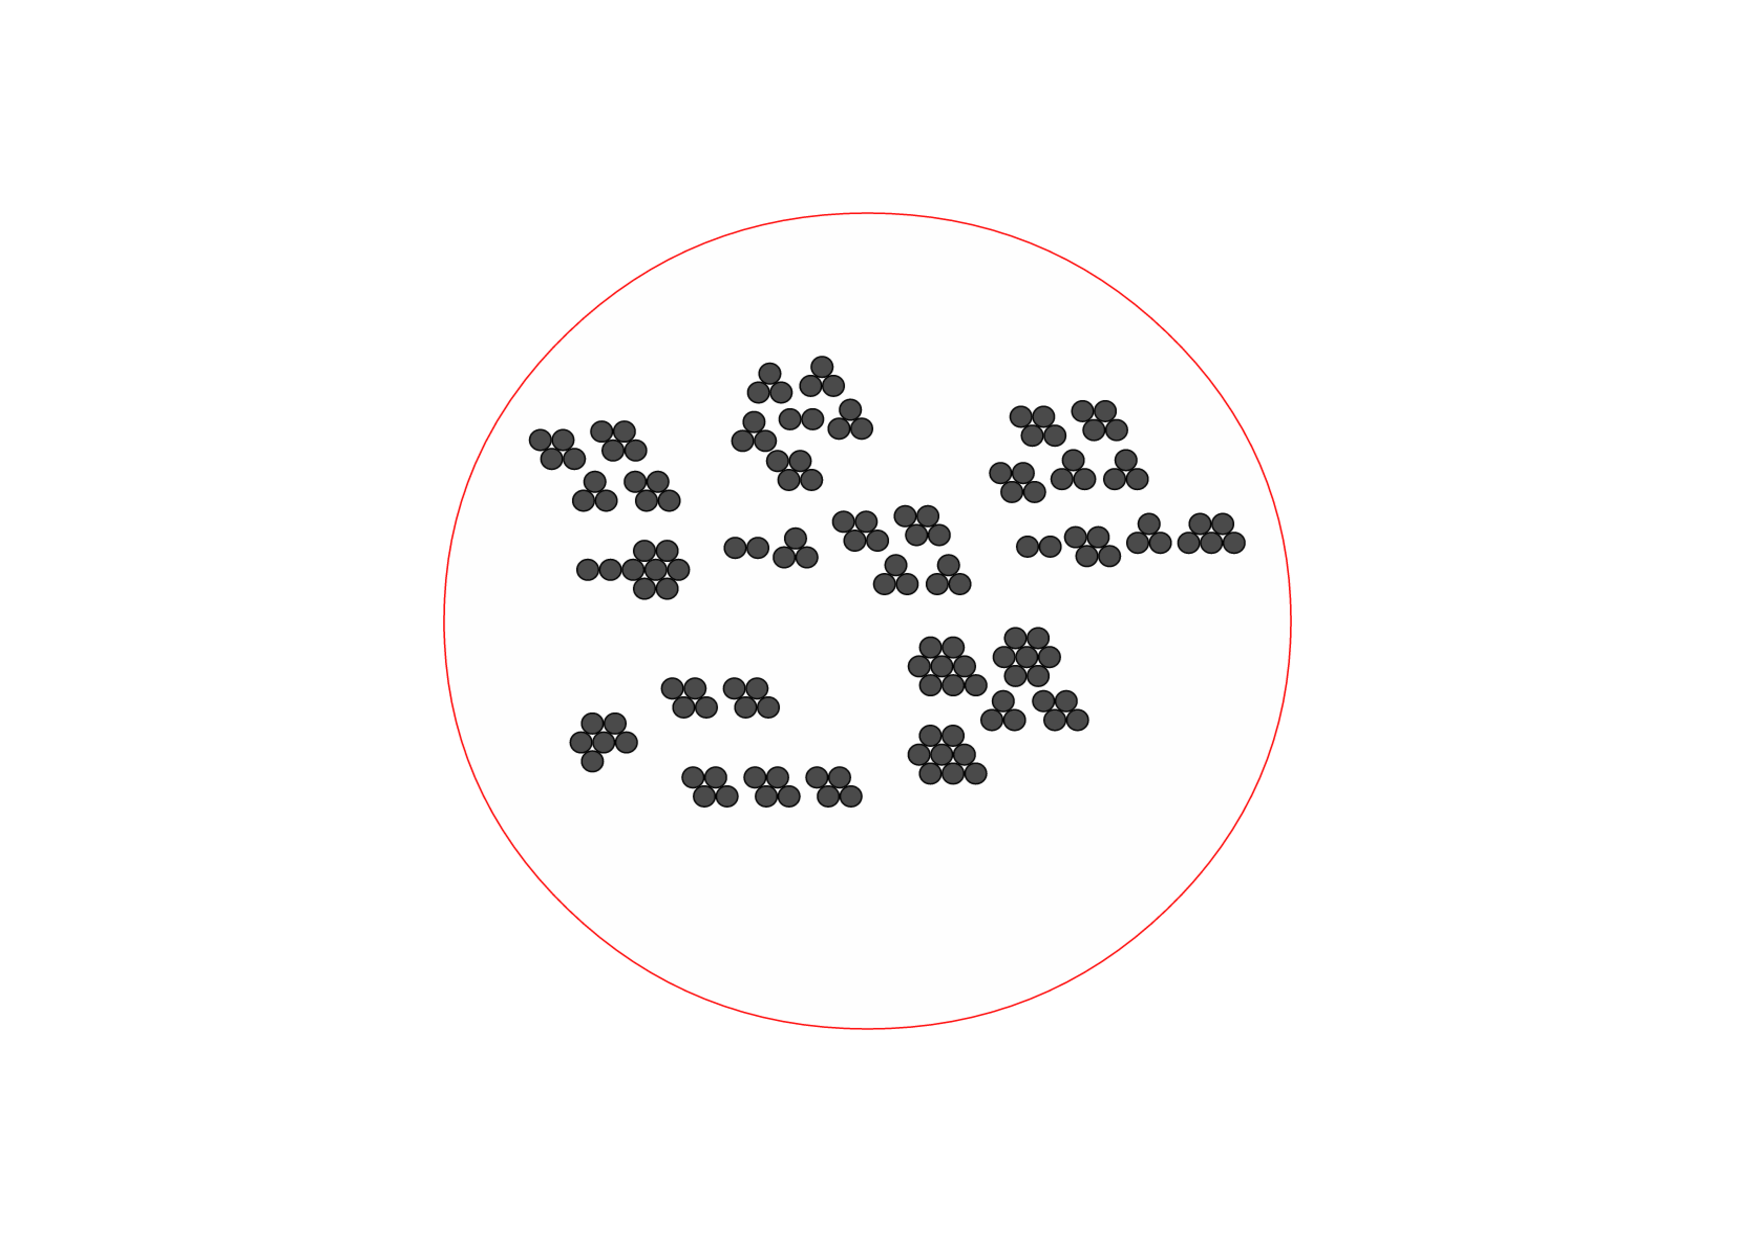
\includegraphics[scale=0.30]{gfx/XP2clean.pdf} 
\end{center}
\caption{\label{figXP2} Full Display (FD) with a non visible hierarchical organization of semantic classes }
\end{figure}

\begin{figure*}[t]
\begin{center}
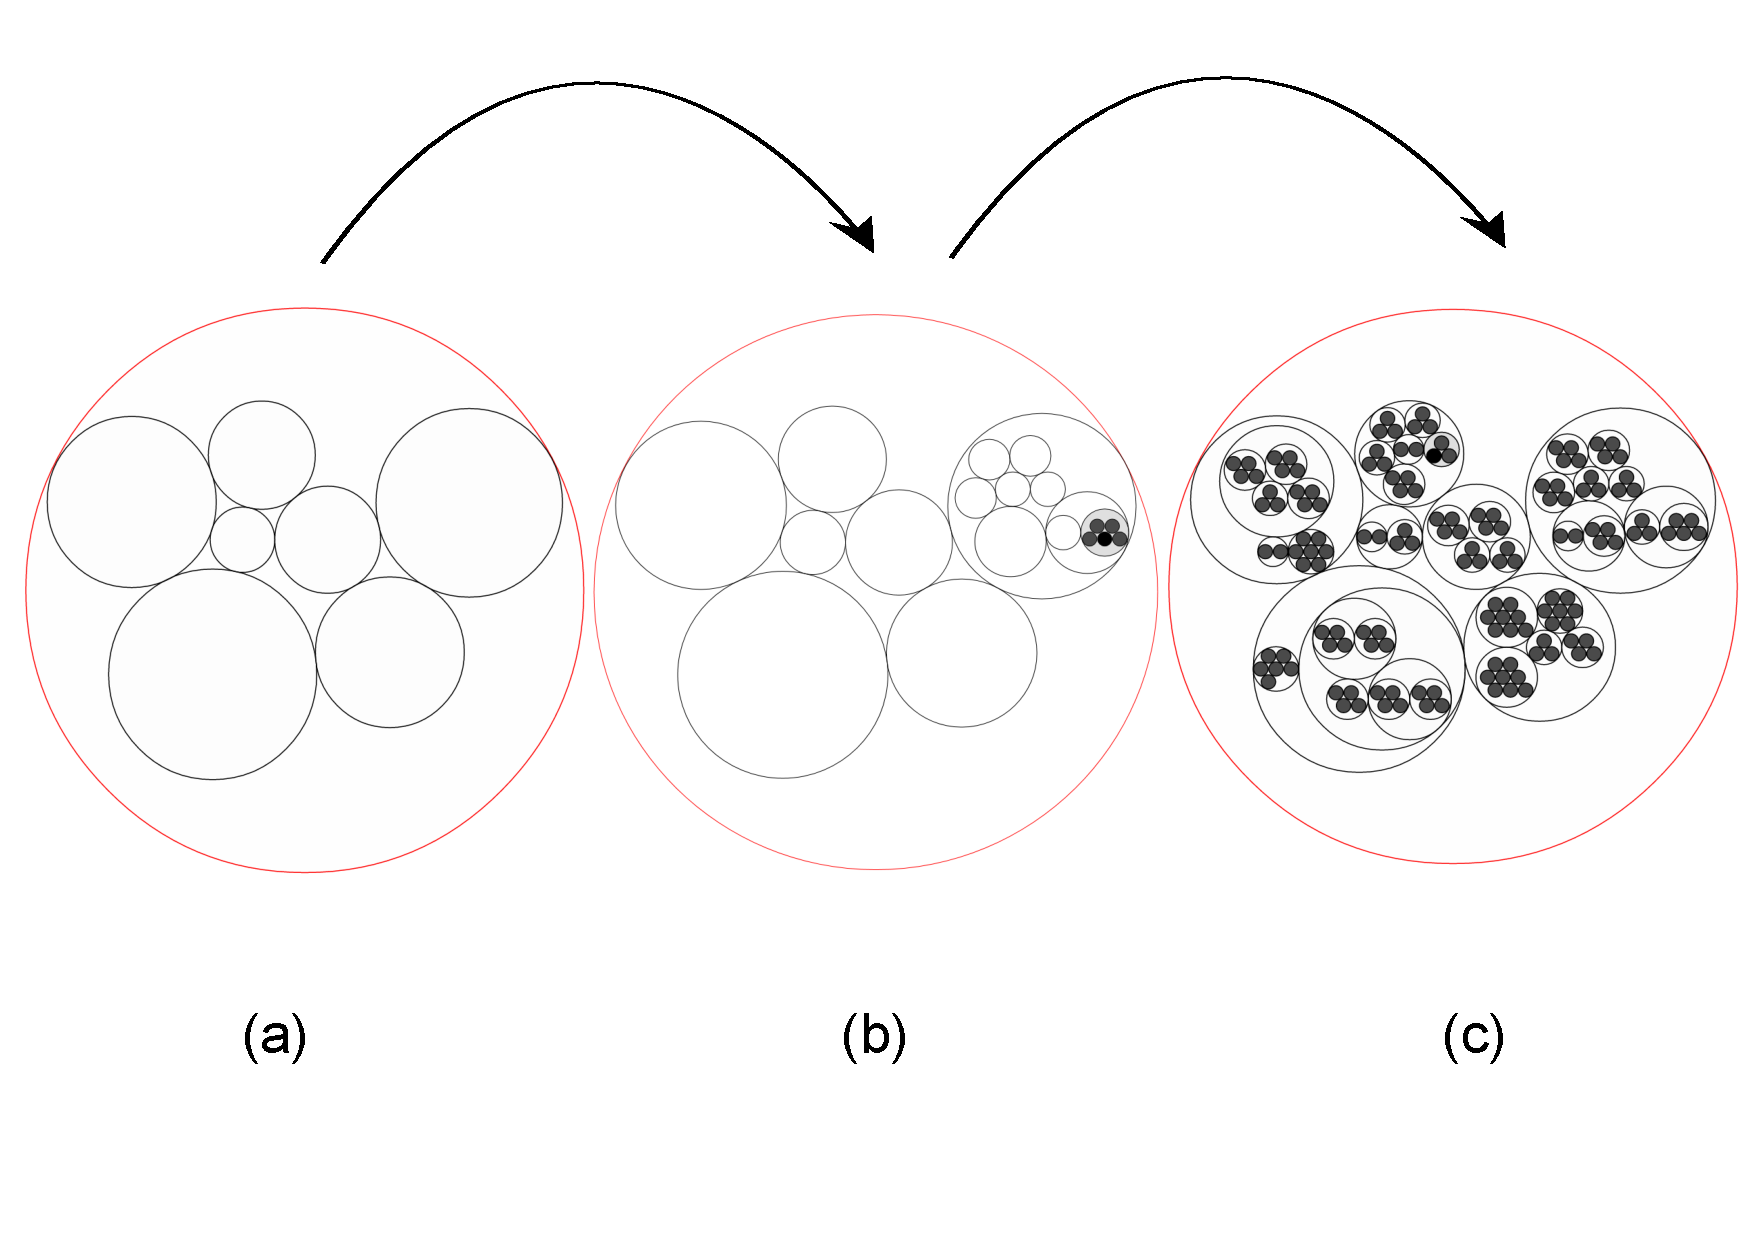
\includegraphics[scale=0.4]{gfx/XP1clean2.pdf} 
\end{center}
\caption{\label{figXP1} Progressive Display (PD) with a  visible hierarchical organization of semantic classes: (a) initial folded version; (b) partly folded version; (c) unfolded version}
\end{figure*}

\begin{figure}[t]
\begin{center}
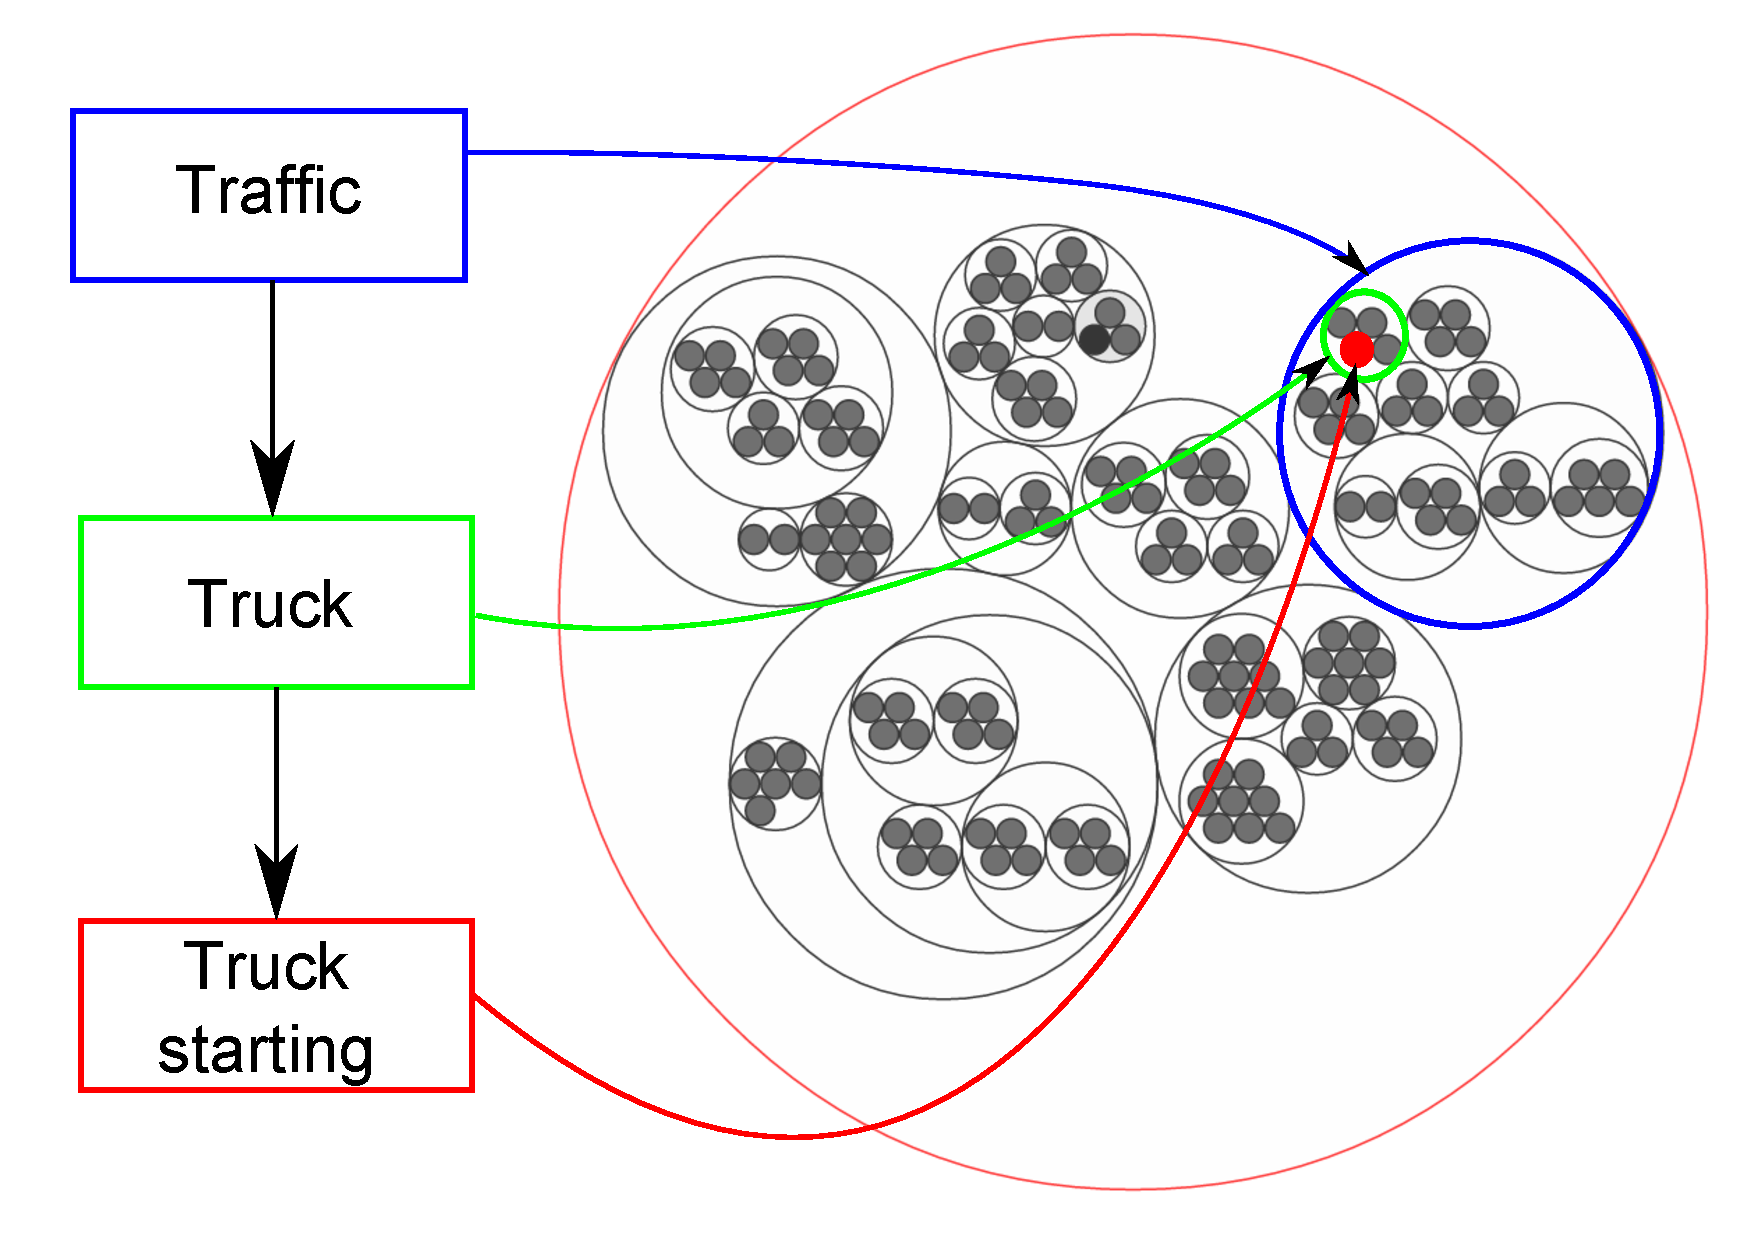
\includegraphics[scale=0.24]{gfx/SSF.pdf} 
\end{center}
\caption{\label{figSSF} Spatial configuration of the Progressive Display (PD) based on the semantic hierarchical structure of the dataset}
\end{figure}

In this section, two listening oriented displays, called respectively Progressive Display (PD) and Full Display (FD) are presented. Both interfaces 1) allow users to explore a sound dataset without any written textual help and 2) base their display upon the hierarchical structure of the dataset. The two interfaces have been designed in order to see whether a progressive top-down display of the hierarchical structure helps the user explore the dataset.

As shown on Figures~\ref{figXP2} and \ref{figXP1}, both interfaces are based on the same principle of distributing in a 2D space the hierarchical structure of the  sound elements of the dataset. Each sound class is represented by a circle. Circles are packed together according to the hierarchical semantic organization of the dataset, as shown on Figure \ref{figSSF}. Thus, subclasses belonging to the same class are close to each others. Circle packing functions of the D3.js (Data-Driven Documents) javascript library \cite{2011-d3} are used to distribute the sound classes in the space. 

The way in which a user visualizes the hierarchical organization varies with the interface:

\begin{itemize}
\item \textit{PD}: users have access to the intermediate semantic levels of the hierarchy. Upon first using PD, they observe circles representing the top classes of the semantic hierarchical structure of the dataset. When users click on a circle, they hear the sound prototype of the class and the subclasses are progressively revealed, represented by white circles contained in the circle that has just been clicked. The same action repeats itself until the user reaches the leaf classes of the hierarchy. The leaf classes are represented with small gray circles, indicating that there is no subclass to discover. Thus the PD has a constrained exploration system. When a user click on a circle, sub-circles are  automatically revealed to him in a gradual way. Each time a sub-circle is automatically revealed, its sound prototype is played. Users may stop the discovery process by clicking on an other circle. 
\item \textit{FD}: users can directly visualize the whole hierarchy, down to the leaf classes. Those leaf classes are distributed  in the same manner as PD. In that sense, the spatial configuration of the unfolded version of PD, which may be obtained after discovering all the classes and subclasses, is similar to that of  FD, as shown on Figures~\ref{figXP2}, \ref{figXP1} and \ref{figSSF}.
\end{itemize}


\section{Experiment} \label{test}

\subsection{Objective}
During this test, three interfaces are compared:
\begin{itemize}
\item PD, which provides a visible hierarchical organization of semantic classes;
\item FD, which provides a non-visible hierarchical organization of semantic classes;
\item an Acoustic Display (AD) providing a 2D representation based on acoustic descriptors. In this case, the spatial configuration is computed by 1) describing the sounds with mel-frequency cepstrum coefficients (MFCCs) and 2) using  a non metric multidimensional scaling with Kruskal's normalized stress to compute sound positions in a 2D space. An example of AD can be seen on~Figure \ref{figXP3}.
\end{itemize}

By comparing PD and FD, the effect of a visible hierarchy on the user is investigated. The goal is to check if forcing the user to browse the high levels of the hierarchy helps him to understand and learn the spatial configuration and the organisation of the sound classes. By confronting PD and FD with AD, the relative efficiencies of semantic based and acoustic based spatial configurations are compared. 

\begin{figure}[t]
\begin{center}
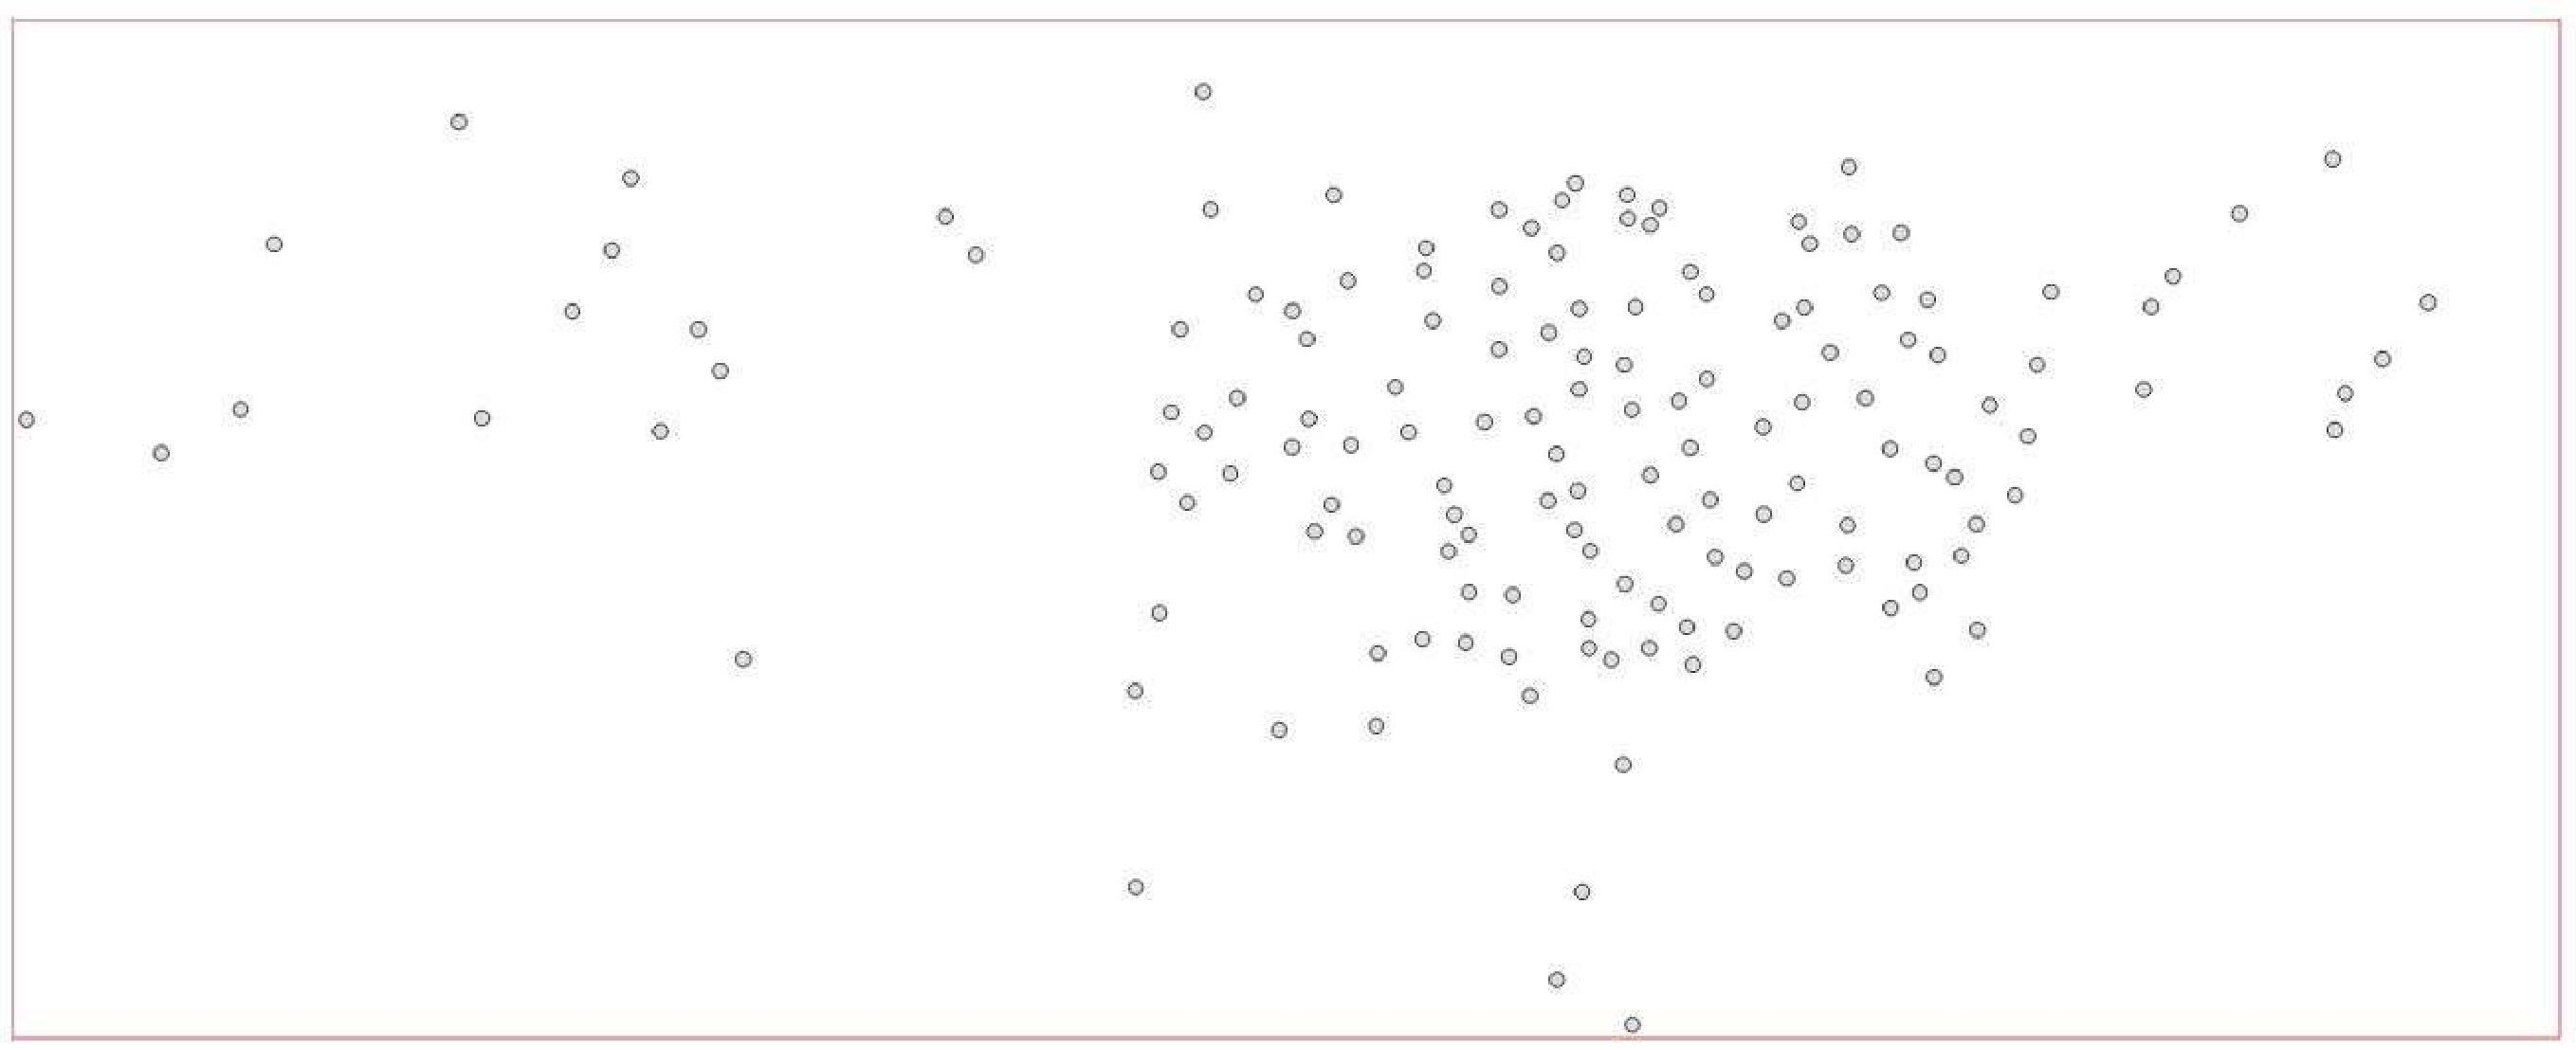
\includegraphics[scale=0.18]{gfx/XP3.pdf} 
\end{center}
\caption{\label{figXP3} The Acoustical Display (AD) computed using  a non metric multidimensional scaling on  MFCCs based acoustic descriptors}
\end{figure}

\subsection{Experimental protocol}
We choose to test and compare the three displays through a crowdsourcing experiment. Here is the link to access the experiment web page \footnote{http://217.70.189.118/soundthings/speedSoundFinding/}.

Subjects are asked to successively retrieve 13 target sounds in a dataset of 149 urban environmental sound events. The target sounds are distributed such as there are at least two target sounds in each top-level class of the semantic hierarchical structure of the dataset. To minimize order effects, target sounds are randomly presented to each subject.

To listen to a target sound, the subject has to click a \textit{Play target sound} button. Subject may replay the target sound  as many times as they like. A timer is started when the subject clicks on a circle for the first time.

When the target sound is found, subject puts an end to its search by clicking on the \textit{Click if found} button. This action 1) stops the timer and 2) loads a new target sound. If the subject does not find the correct target sound, an error message appears, and the experiment continues.

During the experiment, two indications are communicated to the subject:
\begin{itemize}
\item \textit{The research state}: "pause" if the subject is currently not looking for a target sound (at the beginning of the experiment, or between two target sounds);  "in progress"  if the subject is currently looking for a target sound.
\item \textit{Remaining target sounds}: the number of target sounds which remain to find.
\end{itemize}

The experiment ends when all the target sounds have been found.

It is most important to note that PD do not pack up at each target sound search. When a circle is revealed, it remains visible during the whole experiment.



 
\subsection{Data Collection}
Three sets of data are collected during the experiment:
\begin{itemize}
\item the total duration of the entire experiment. It includes breaks between two target sound searches and it is called the \textit{absolute duration}.
\item the duration of each search. The sum of the 13 duration searches, which is the \textit{absolute duration} minus the break times between two target sound searches, is called \textit{the relative duration}.
\item the name of each sound which has been heard.
\item the time at which each sound has been heard.  
\end{itemize}



\subsection{Apparatus}
A crowd sourcing approach has been adopted. The experiment was designed to be supported by the  \textit{chrome-browser} web navigator. The link to the experiment has been sent to the subjects via three  mailing list being \textit{music-ir, auditory} and \textit{uuu-IRCAM} (internal IRCAM mailing list). Subjects were allowed to perform the experiment once, and on one interface only. Data were automatically collected server-side at the end of the experiment. Subjects were asked to use headphones. All the presented sounds were normalized to the same root mean square (RMS) level.
\subsection{Participants}
60 subject have completed the experiment, 20 for each interface.

\section{Results} \label{results}
\subsection{Outlier detection}
Outlier detection is an important step of any crowdsourcing experiment as experimenters do not control the experimental environment in which the subjects perform the experiment \cite{komarov2013crowdsourcing}\cite{buchholz2011crowdsourcing}. A widely used method to detect outlier in  human-computer interaction studies is to consider as outlier an observation  which deviates of at least $\pm2$ standard deviation ($STD$) from the average \cite{komarov2013crowdsourcing}. As this method is not robust to the presence of isolated extreme observations (as it is often the case for crowdsourcing experiment), a method using the inter-quartile range ($IQR$) proposed by \cite{komarov2013crowdsourcing} is used in this paper. With this approach, an observation is considered to be an outlier if it is more than $3*IQR$ higher than the third quartile or more than $3*IQR$ lesser than the first quartile. For normalized distribute data, the $IQR$ method remove less than 0.00023\% of the data whereas the  $STD$ method remove 4.6\% of the data \cite{komarov2013crowdsourcing}. This methods is applied to the following list of parameters:

 \begin{table}[t]
\caption{\label{tab1} Standard deviations of the number of heard sounds per subject, with and without outliers.}
\begin{center}
\begin{tabular}{cccc}
Interface &  PD &  FD& AD \\
\hline
with outliers & 141 & 155 & 315 \\
without outliers & 139 & 140 & 146 \\  
\hline
\end{tabular}
\end{center}
\end{table} 
\begin{table}[t]
\caption{\label{tab2} Standard deviations of the \textit{relative duration} per subject, with and without outliers.}
\begin{center}
\begin{tabular}{cccc}
Interface &  PD &  FD &  AD \\
\hline
with outliers & 353 & 277 & 520 \\
without outliers & 363 & 249 & 273 \\  
\hline
\end{tabular}
\end{center}
\end{table} 

\begin{table}[t]
\caption{\label{tab3} Standard deviations of the \textit{absolute duration} per subject, with and without outliers.}
\begin{center}
\begin{tabular}{cccc}
Interface &  PD &  FD &  AD \\
\hline
with outliers & 1401 & 339 & 4034 \\
without outliers & 408 & 327 & 273 \\  
\hline
\end{tabular}
\end{center}
\end{table}


\begin{itemize}
\item durations of  each target sound search
\item average duration of target sound searches
\item maximum duration of target sound searches
\item \textit{relative duration}
\item \textit{absolute duration}
\item number of heard sounds for each target sound search
\item average number of heard sounds
\item maximum number of heard sounds
\item total number of heard sounds
\end{itemize}

Using the $IQR$ method, 4 subjects are detected as outliers and removed from the analysis. 1 subject used PD, 1 subject FD, and 2 subjects AD. 2 subjects are detected by observing the \textit{absolute duration} (4 and 12 hours), 1 subject by observing the total number of heard sounds (1800 heard sounds, roughly 12 times the total size of the corpus) and 1 subject by observing the number of heard sound for the first target sound search (321 heard sounds, including 21 times the target sound).

The tables \ref{tab1}, \ref{tab2} and \ref{tab3} measure the effect of the presence of the  outliers on the standard deviations of three observed data being the total number of heard sounds, the \textit{relative duration} and the \textit{absolute duration}. The removal of the outliers have important effects on the data distributions, specially for AD.

\begin{figure}[t]
\begin{center}
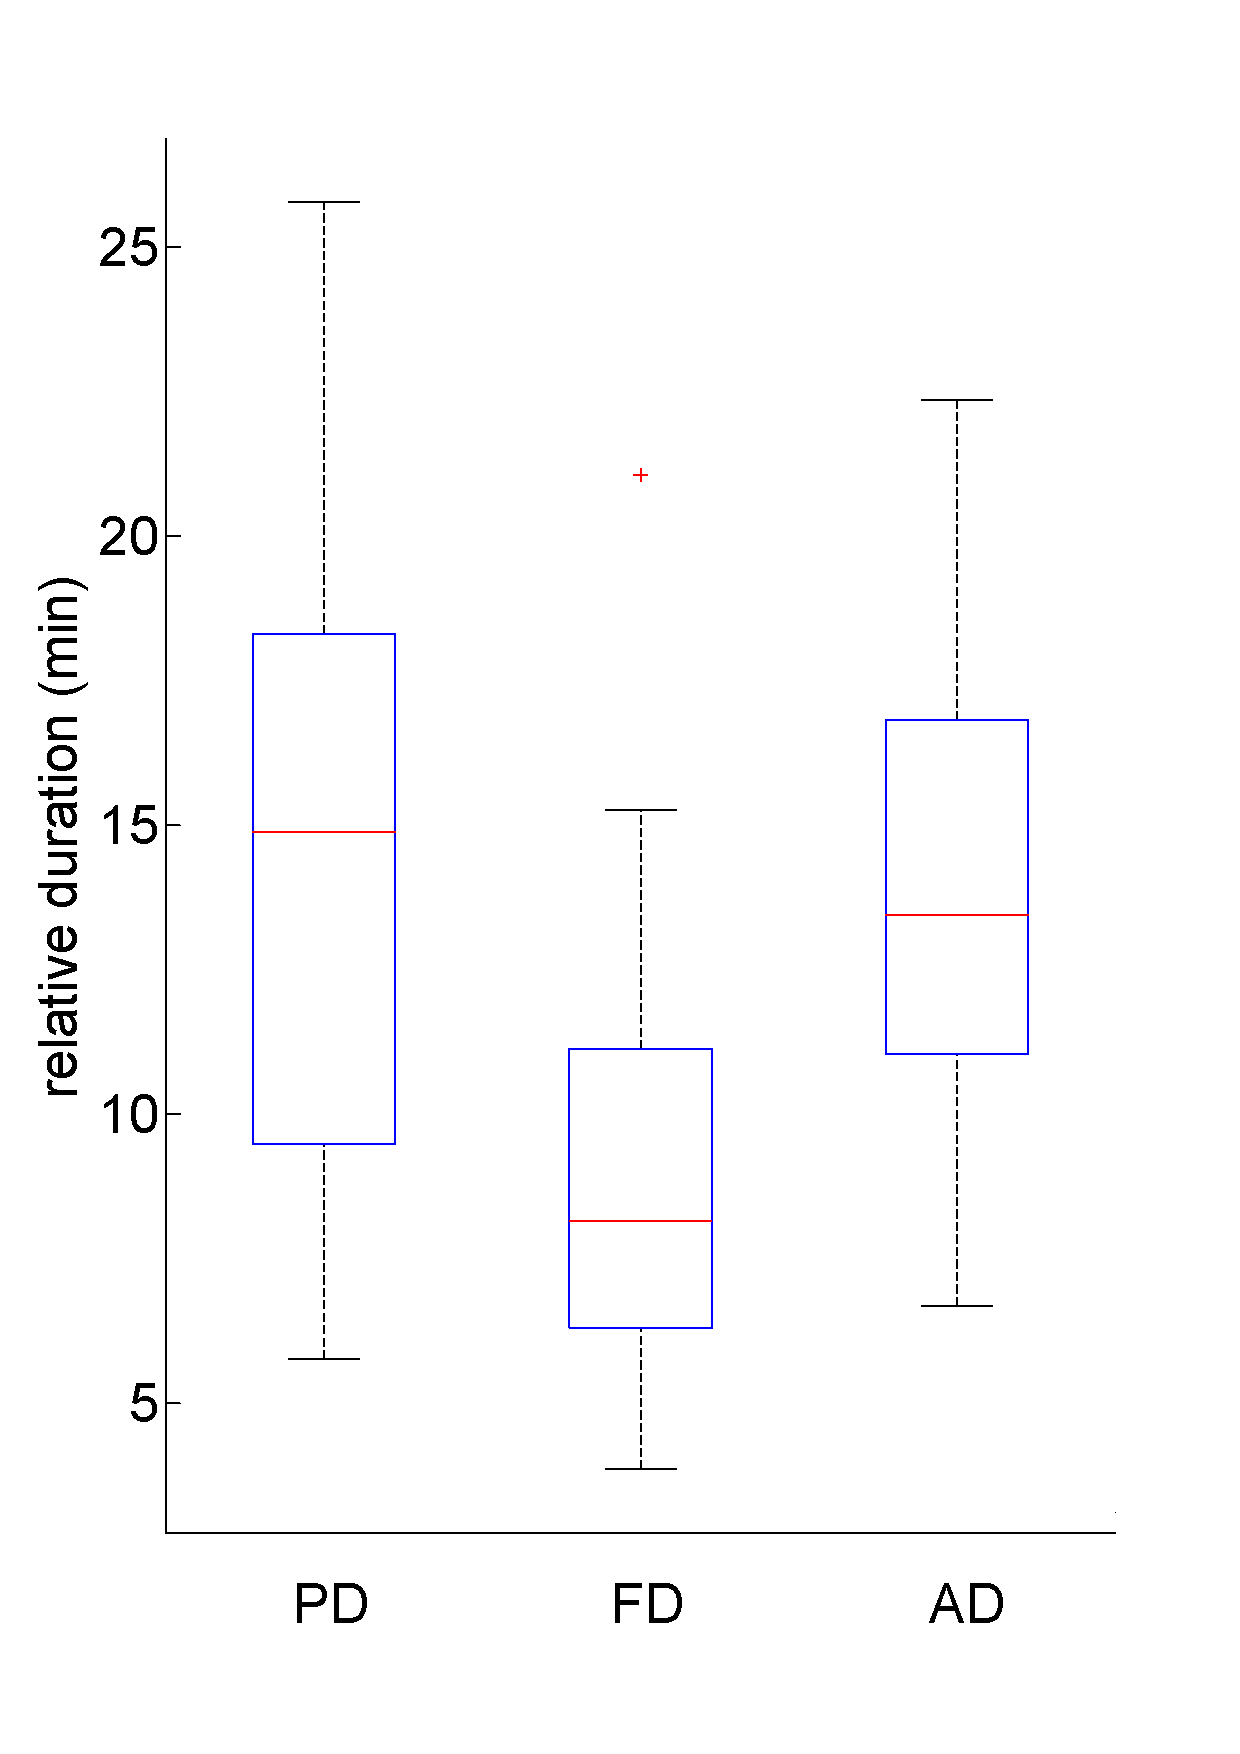
\includegraphics[scale=0.36]{gfx/RDbis.pdf} 
\end{center}
\caption{\label{fig1} Boxplot representing the distributions of the relative durations for the PD, FD and AD}
\end{figure}  

\begin{figure}[t]
\begin{center}
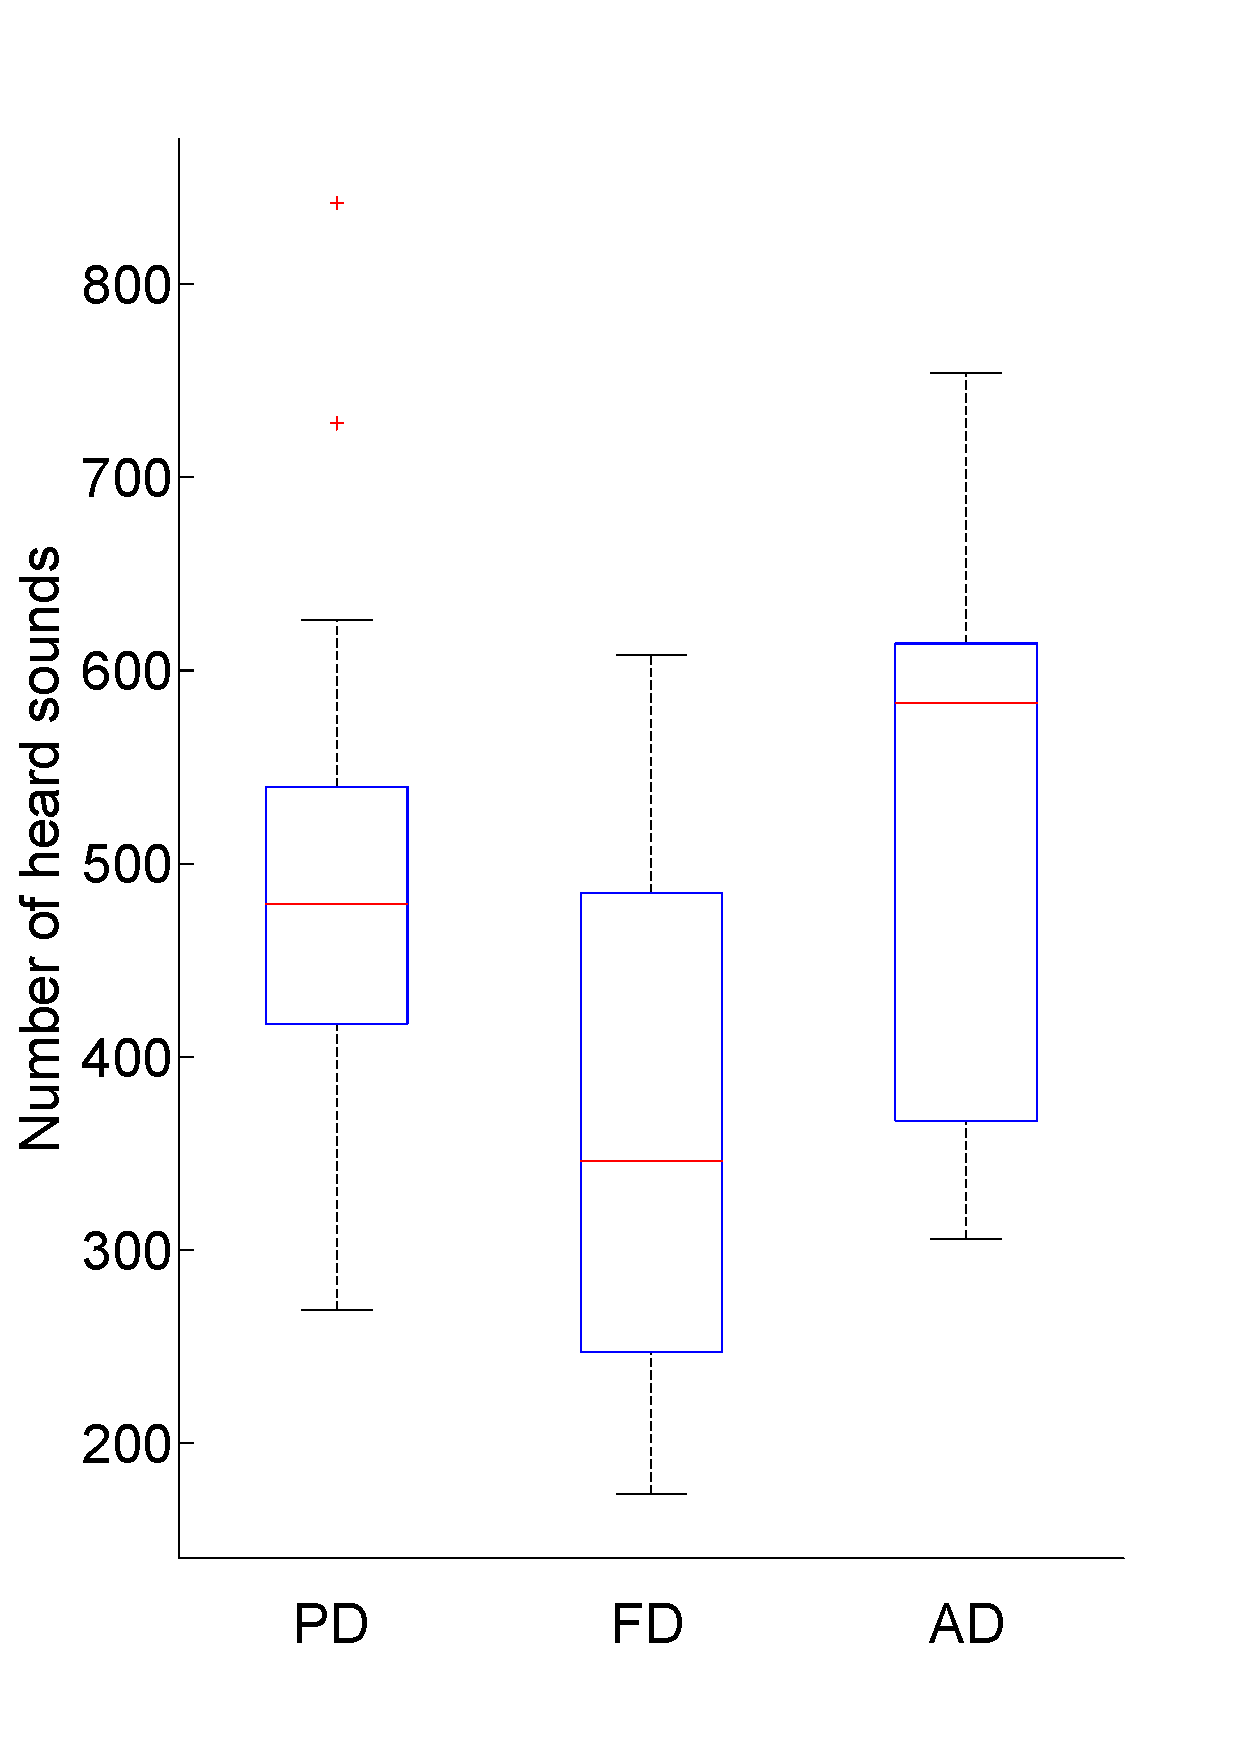
\includegraphics[scale=0.36]{gfx/NBRbis.pdf} 
\end{center}
\caption{\label{fig2} Boxplot representing the distributions of the numbers of heard sounds for the PD, FD and AD}
\end{figure}


\subsection{Interface efficiencies}

To characterize the displays efficiencies, three set of collected data are assessed: 
\begin{itemize}
\item the \textit{relative duration} 
\item the number of heard sounds 
\item the number of heard sounds without duplication. By "without duplication" we mean that, if a same sound prototype is heard 10 times during the 13 searches of the  experiment, it counts only for one. 
\end{itemize}

The two first data help us qualify the notion of efficiency by considering the time and the number of clicks needed to achieve the task (ie. reach the target). The goal for those values is to be as low as possible. The third data allows us to measure the selectivity of the interfaces. A low number of heard sounds without duplication indicates that subjects understood the spatial organisation of the dataset, and use this knowledge to improve their searches. In contrary, a high number of heard sounds without duplication suggest that the subject did not understood the way circles are organized in space, and tends to play all the sounds at each search. The maximum number of heard sounds without duplication is the corpus size: 149 sounds.


Concerning the \textit{relative durations}, distributions of the data are displayed on Figure~\ref{fig1} for the three interfaces. FD seems to  perform better  than the other interfaces, whereas PD and AD seem to have similar results. To refine the analysis, a two sided Wilcoxon rank sum test is considered. It is a non parametric statistical test which tests the null hypothesis that two set of observed data originate from distributions having equal median \cite{gibbons2011nonparametric}. As expected, FD is significantly better than the other interfaces (FD-PD: $p=0.0142$; FD-AD: $p=0.028$) and there is no statistical differences between PD and AD (PD-AD: $p=1$). 

Distributions of  the numbers of heard sounds are displayed on Figure~\ref{fig2} for the three interfaces. Results are similar of those observed for the \textit{relative durations}. FD significantly outperforms the other interfaces (FD-PD: $p=0.0115$; FD-AD: $p=0.018$), whereas PD and AD show similar outcomes (PD-AD: $p=0.3699$).

Lastly, Figure~\ref{fig3} displays the distributions of the number of heard sounds without duplication. This time the results of AD are significantly lower than those of both PD and FD (AD-PD: $p=8.4910.10^{-4}$; AD-FD: $p=0.027$).  For AD, 75\% of the subjects heard more than 138 sounds, and 25\% heard 148 sounds, that is almost the entire database. Considering PD, 75\% of subjects heard  less than 133 sounds, against 144 for FD. There is no statistical differences between the PD and FD (PD-FD: $p=0.8607$), indicating that those two interfaces perform equally.

\begin{figure}[t]
\begin{center}
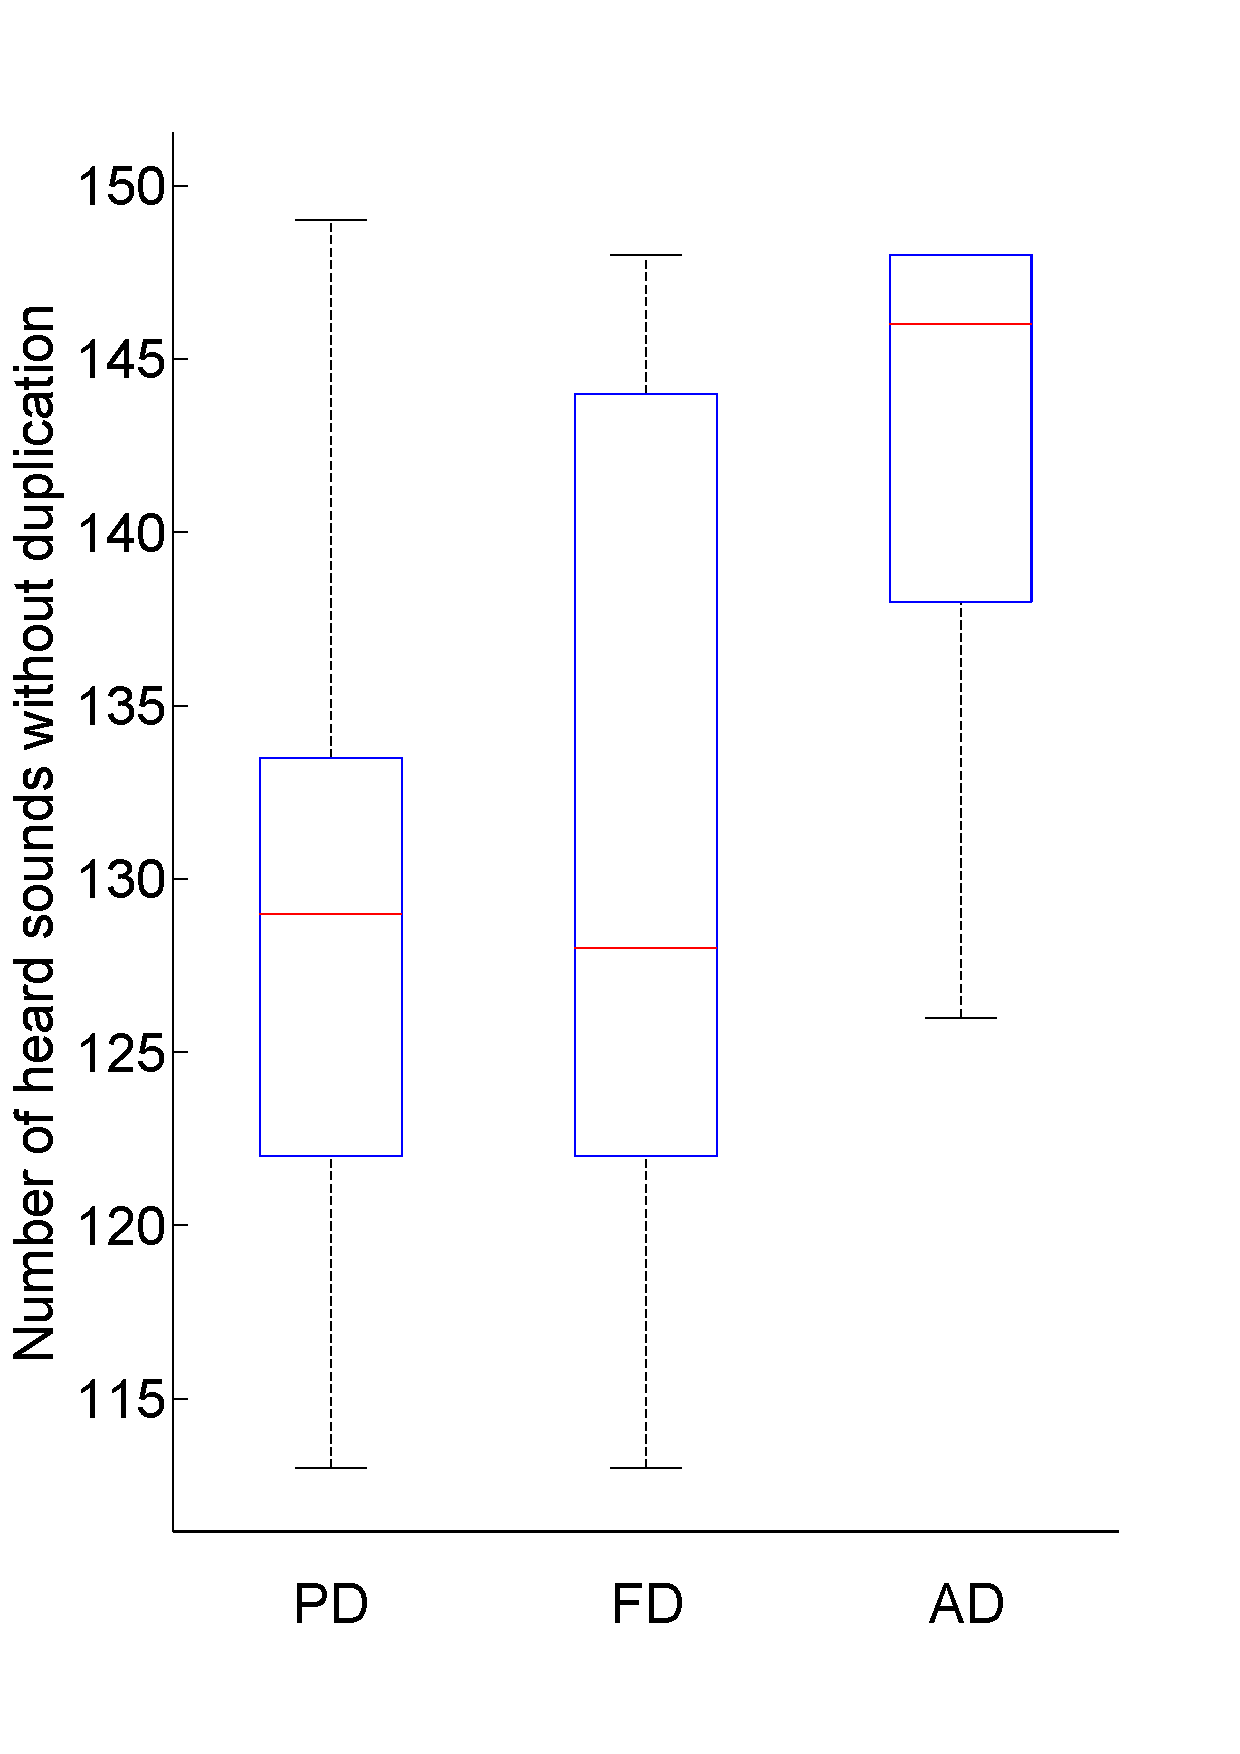
\includegraphics[scale=0.36]{gfx/SDbis.pdf} 
\end{center}
\caption{\label{fig3} Boxplot representing the distributions of the numbers of heard sounds without duplication for the PD, FD and AD}
\end{figure}

According to those results, a hierarchical organization of the dataset based on semantic values (PD and FD) allows users to retrieve the 13 target sounds 1) quicker, and 2) by listening to a smaller amount of sounds than an organization based on acoustic descriptors (AD). But those two effects are significantly compromised when users have to parse the entire hierarchy to reach the first target sound, as it the case for PD. It seems that imposing a graphical representation of the hierarchy disturbs or confuses the user instead of allowing him to learn the spatial organization of the classes. 
%The semantic-based spatial organization allow users to significantly improve the precision of their searches, by clicking on less different circles, irrespective of whether or not the hierarchy is imposed. 

\newpage


\subsection{Learning phenomenon}

We now study if and how users  progressively acquire knowledge about the spatial organization of the classes. To do that, variations of the data over the searches are assessed. Three sets of collected data are used:

\begin{itemize}
\item the duration of each target sound search 
\item the number of heard sounds for each target sound search 
\item the number of heard sounds for each target sound search without duplication. 
\end{itemize}

Figure \ref{fig1PR} (bottom) displays the evolution of the medians of the durations of each target sound search observed over the subjects for PD, FD and AD. It is interesting to note that both for PD and FD, the maximum value is observed for the first search, whereas it is observed for the fourth search for AD. Moreover if the curve profiles of PD and FD  seem to progressively decrease and are very similar, the one of AD is much more irregular. If we compare PD and FD, we note  that the durations are systematically shorter for FD, except for the search 12. Furthermore, for FD, a threshold of 25 seconds is reached from the search four,  whereas it is of 50 seconds for PD. 

\begin{figure}[t!]
\begin{tabular}{c}
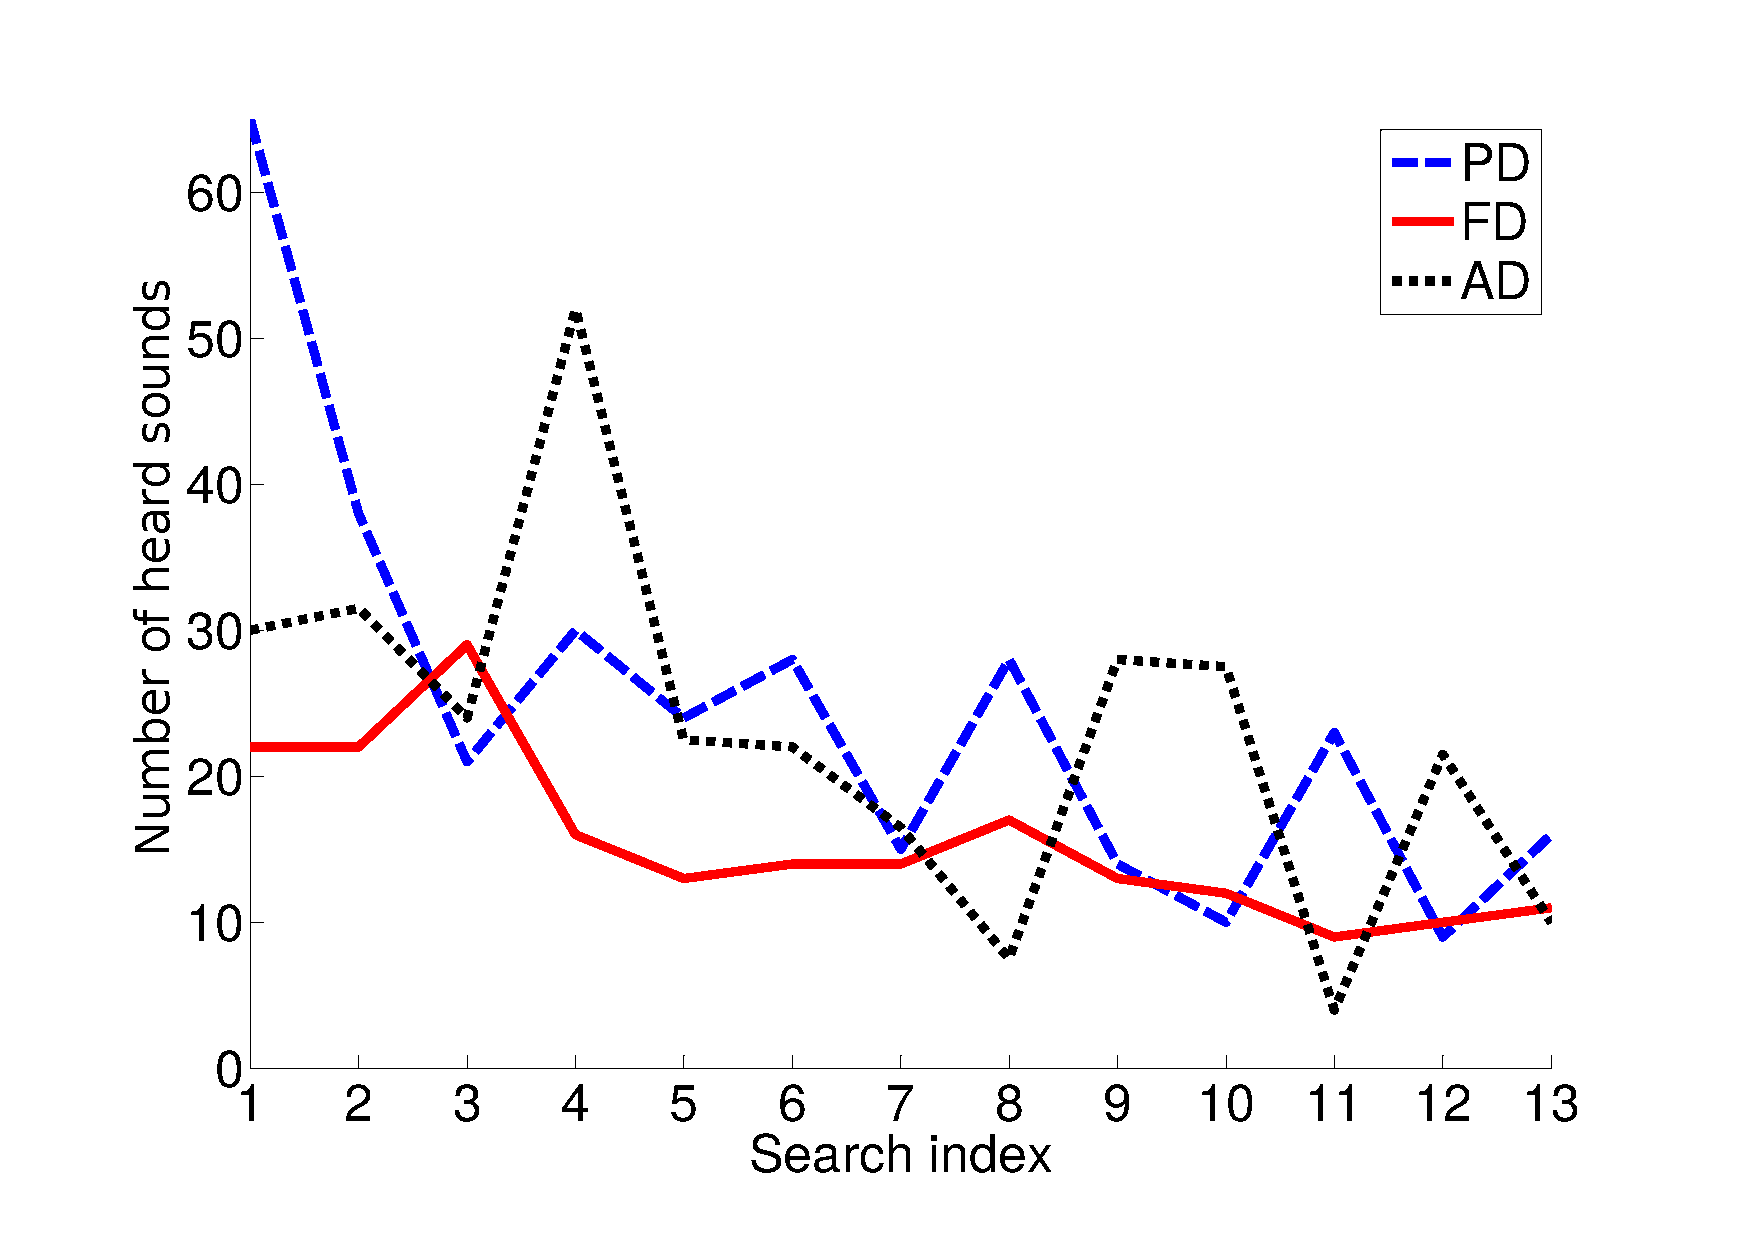
\includegraphics[scale=0.29]{gfx/NOHS.pdf} \\
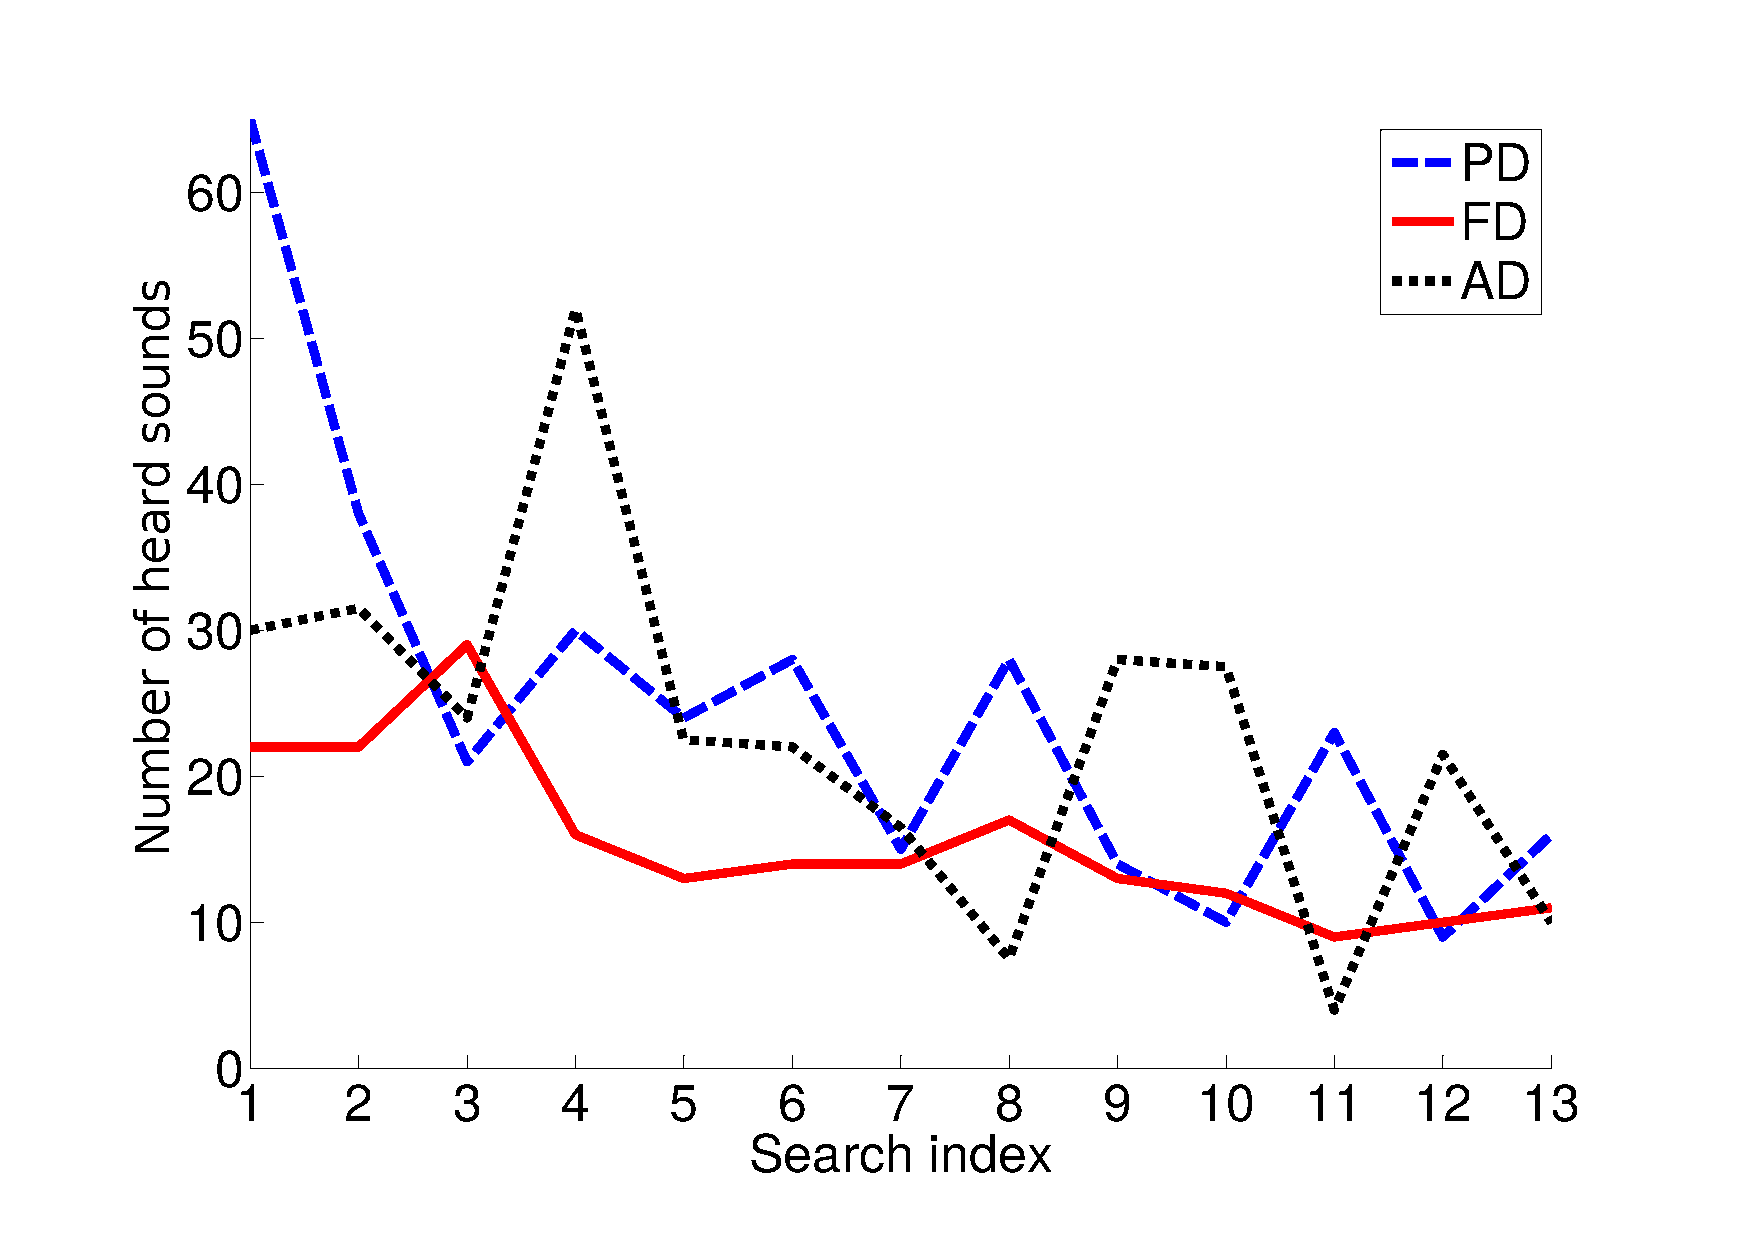
\includegraphics[scale=0.29]{gfx/NOHS.pdf} \\ % should be WD
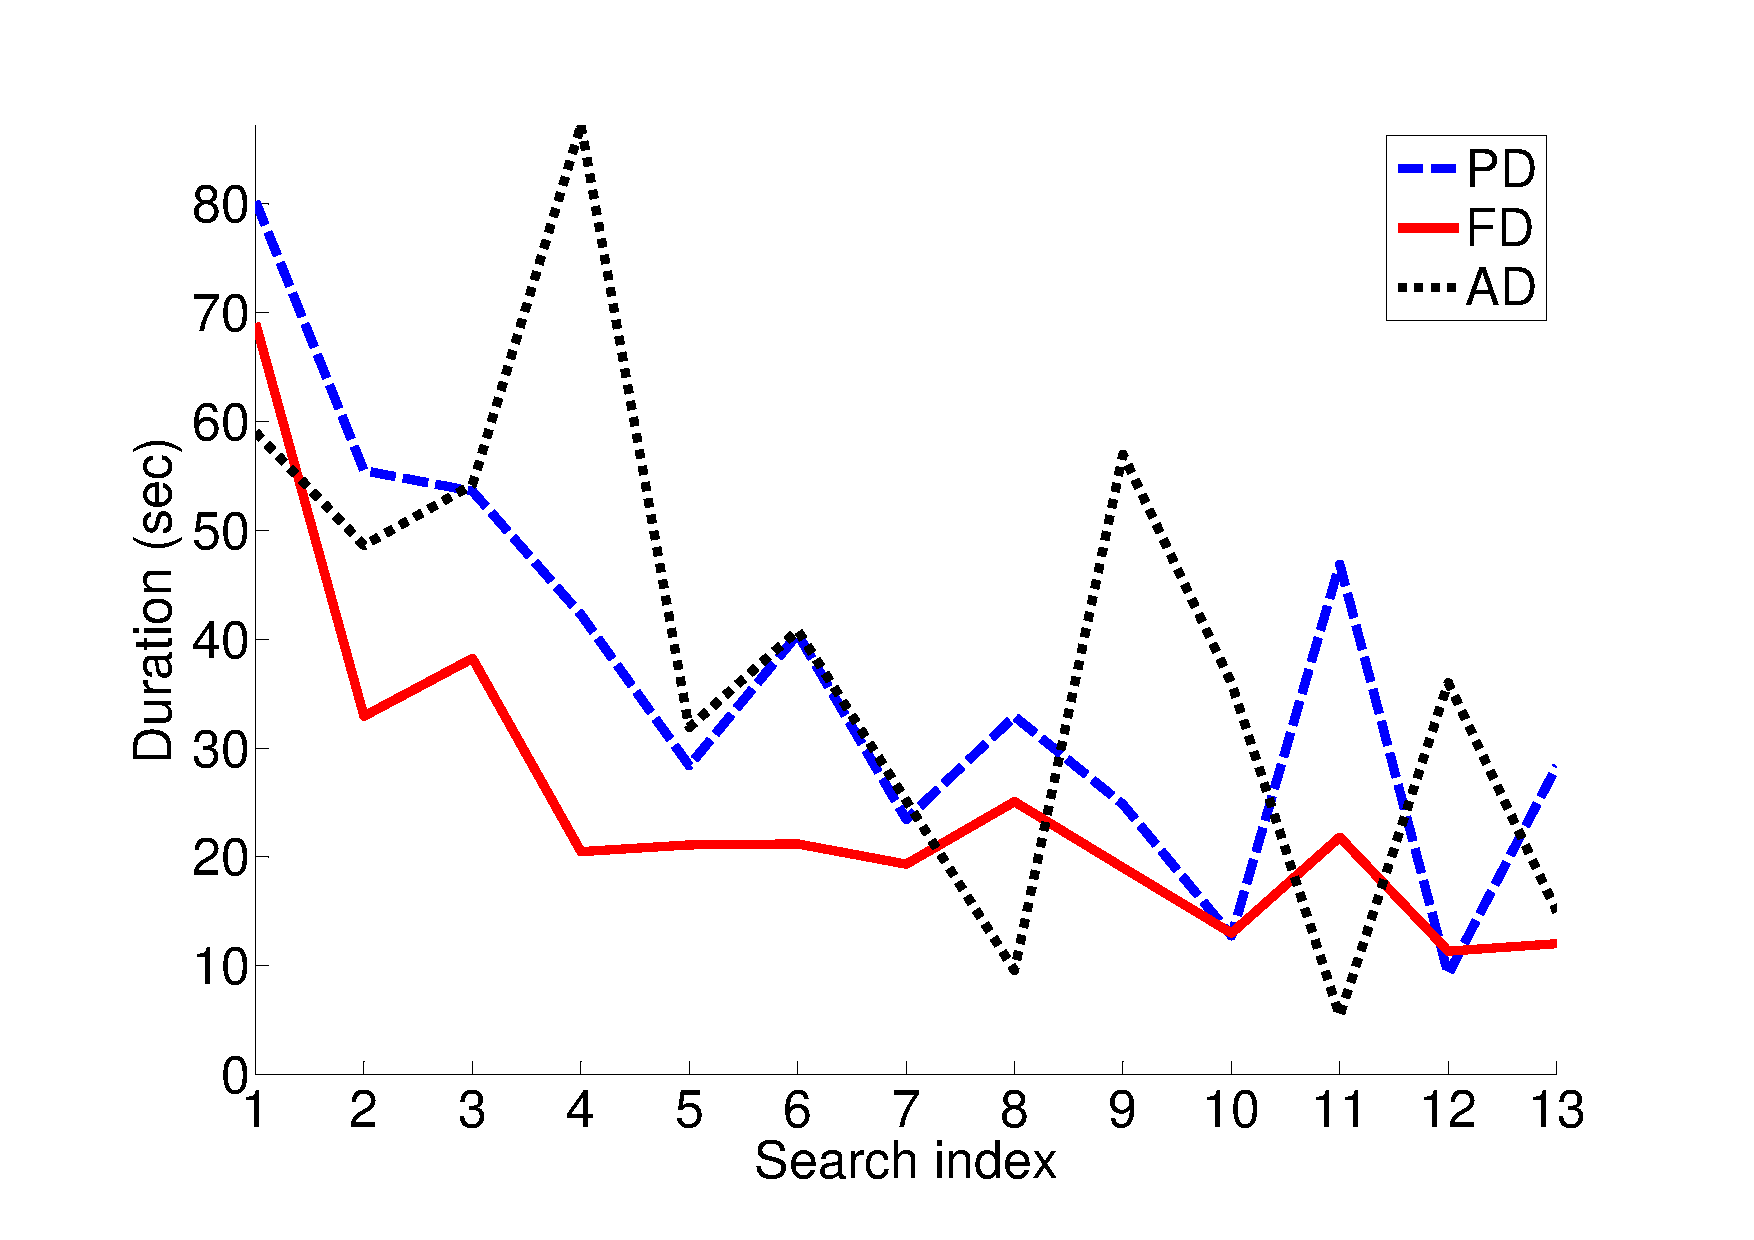
\includegraphics[scale=0.29]{gfx/duration.pdf} 
\end{tabular}
\caption{\label{fig1PR} Medians of (top) the numbers of heard sounds at each target sound search, (middle) the numbers of heard sounds without duplication (WD) at each target sound search, (bottom) the relative durations at each target sound search \gregoire{peux-tu ajouter WD.pdf ? la deuxieme figure}}
\end{figure}
%\begin{figure}[t]
%\begin{center}
%\includegraphics[scale=0.38]{gfx/nbrPR.pdf} 
%\end{center}
%\caption{\label{fig2PR} Medians of the numbers of heard sounds at each target sound search (abscissa) for the PD (top), FD (middle) and AD (bottom)}
%\end{figure}
%\begin{figure}[t]
%\begin{center}
%\includegraphics[scale=0.38]{gfx/sdPR.pdf} 
%\end{center}
%\caption{\label{fig3PR} Medians of the numbers of heard sounds without duplication at each target sound search (abscissa) for the PD (top),  FD (middle) and AD (bottom)}
%\end{figure}
Figure \ref{fig1PR} (top) displays the evolution of the medians of the numbers of heard sounds for each target sound search, observed over the subjects for the three interfaces. If the curve profiles of PD and AD seem to be similar to those respectively observed for the durations, here the maximum value for FD  is reached for the third search. Again, values of FD are mostly below those of PD, except for the search index 3,10 and 12. For both PD and FD the curves oscillate from the search four, but those oscillations occur in a range of $9-17$ for FD and  $9-30$ for PD. Similar results are found for the evolution of the medians of the numbers of heard sounds without duplication, shown on Figure \ref{fig1PR} (middle).

Those results tend to indicate that PD and FD facilitate the learning of the spatial configuration, as the search durations and the numbers of heard sounds at each search decrease over time. Although curves for PD and FD have similar profiles, FD seem to better perform as users of FD where able to find the target sounds faster by clicking on fewer circles.

\section{Conclusion}

In this paper, two displays allowing users to explore a sound dataset without written textual help are presented. The interfaces distribute sounds represented by circles on a 2D space. The spatial organisation is driven by semantic features. The two graphical displays are assessed and compared to a third listening based interface in which spatial configuration depends upon acoustic features. The tests consist in data retrieval tasks. 
The Full-Display (FD), that allows users to directly visualize the leaf classes of the semantic hierarchical structure, proves to be the most effective interface for the task.

Two main conclusions may be derived from this experiment. First, a spatial configuration based on semantic features is more effective to retrieve target sounds than a spatial configuration based on acoustic features. Second, an imposed visualisation of the semantic hierarchical structure of the dataset does not help user to understand and learn the spatial configuration of the semantic class, but instead disturbs the navigation. 


%It has to be noted that the test datasets are relatively small in terms of leaf sound classes. It may be interesting to test the FD on a larger dataset. 
%
%To conclude, if this study goal was to investigate the viability of an audio based data mining interface, other studies addressing comparison between FD and keyword based interfaces remain to be conducted. 


\section{Acknowledgements}

Research project partly funded by ANR-11-JS03-005-01.

\bibliographystyle{abbrv}
\bibliography{sigproc}  % sigproc.bib is the name of the Bibliography in this case

%In particular, much consideration has been given in order to avoid any semantic bias. Indeed any selection process based on keyword searching would have influenced the subject choices, and makes impossible or inadvisable to run any kind of identification tasks. 
%
%In a previous study \cite{ssf} we found  that the perceptively inspired structured of the sound data set (on which depends the spatial configuration of the circles) offers a easy-to-navigate format that allows subject to quickly understand the spatial localization of the different sound element classes and thus  enable them to quickly find a sound after a short amount of time. 
%
%%The interface selection has been tested in a previous \textit{crowd-sourcing} experiment on 60 subject. The goal was to find 10 target sound. Results showed that this interface allows subject to learn the sound spatial organisation, and to quickly retrieve a sound after some trials. 
\end{document}
